\documentclass{beamer}
\usetheme[nomail, amurmapleblue]{Amurmaple}

\usepackage{amsfonts,amsmath,amssymb,amsthm}
\usepackage{xcolor}
\usepackage{graphicx,wrapfig}

\usepackage{hyperref}
\hypersetup{
    colorlinks=true,
    citecolor=blue,    % Citation color
    linkcolor=red,     % Internal document links
    urlcolor=magenta   % URL and web links
}

\usepackage{tikz}
\usetikzlibrary{decorations.pathreplacing, shapes.geometric}
\usepackage{booktabs}

% ========================
% Additional commands
\newcommand{\prob}{\mathbb{P}}
\newcommand{\E}{\mathbb{E}}
\newcommand{\tr}{^\top}
\newcommand{\trace}{\mathrm{trace}}
\newcommand{\bb}[1]{\boldsymbol{#1}}
\newcommand{\bbhat}[1]{\hat{\boldsymbol{#1}}}
\newcommand{\norm}[1]{\left\lVert#1\right\rVert}
\DeclareMathOperator*{\argmin}{arg\,min}

\newcommand{\blue}[1]{\textcolor{blue}{#1}}
\newcommand{\todo}[1]{\textcolor{red}{TODO: #1}}



% ==========================
% Preamble

\title[WISER]{\Large{Robust determination of the number of factors via divergence information criteria}}
\author[S.~Roy]{Subhrajyoty Roy} 
\mail{roy.s@wustl.edu}
\collaboration{in collaboration with \textbf{Abhik Ghosh} and \textbf{Ayanendranath Basu}}

\institute[EcoSta]{EcoSta 2026} 

\date{Aug 8, 2026} 


% ==========================

\begin{document}

\maketitle

\thanksframe{Motivation}

\begin{frame}{Cross-Country Sovereign Bond Yields}
    
    \begin{itemize}
        \item It is well known that the yields of sovereign bonds across countries are highly correlated.
        \item There are typically a few macroeconomic (global) factors that drive the yields of sovereign bonds across countries.
        \item Let's look at some recent data (on daily yields of $10$ year bonds) to see if this is indeed the case!
    \end{itemize}

\end{frame}


\begin{frame}{Cross-Country Soverign Bond Yields}
    
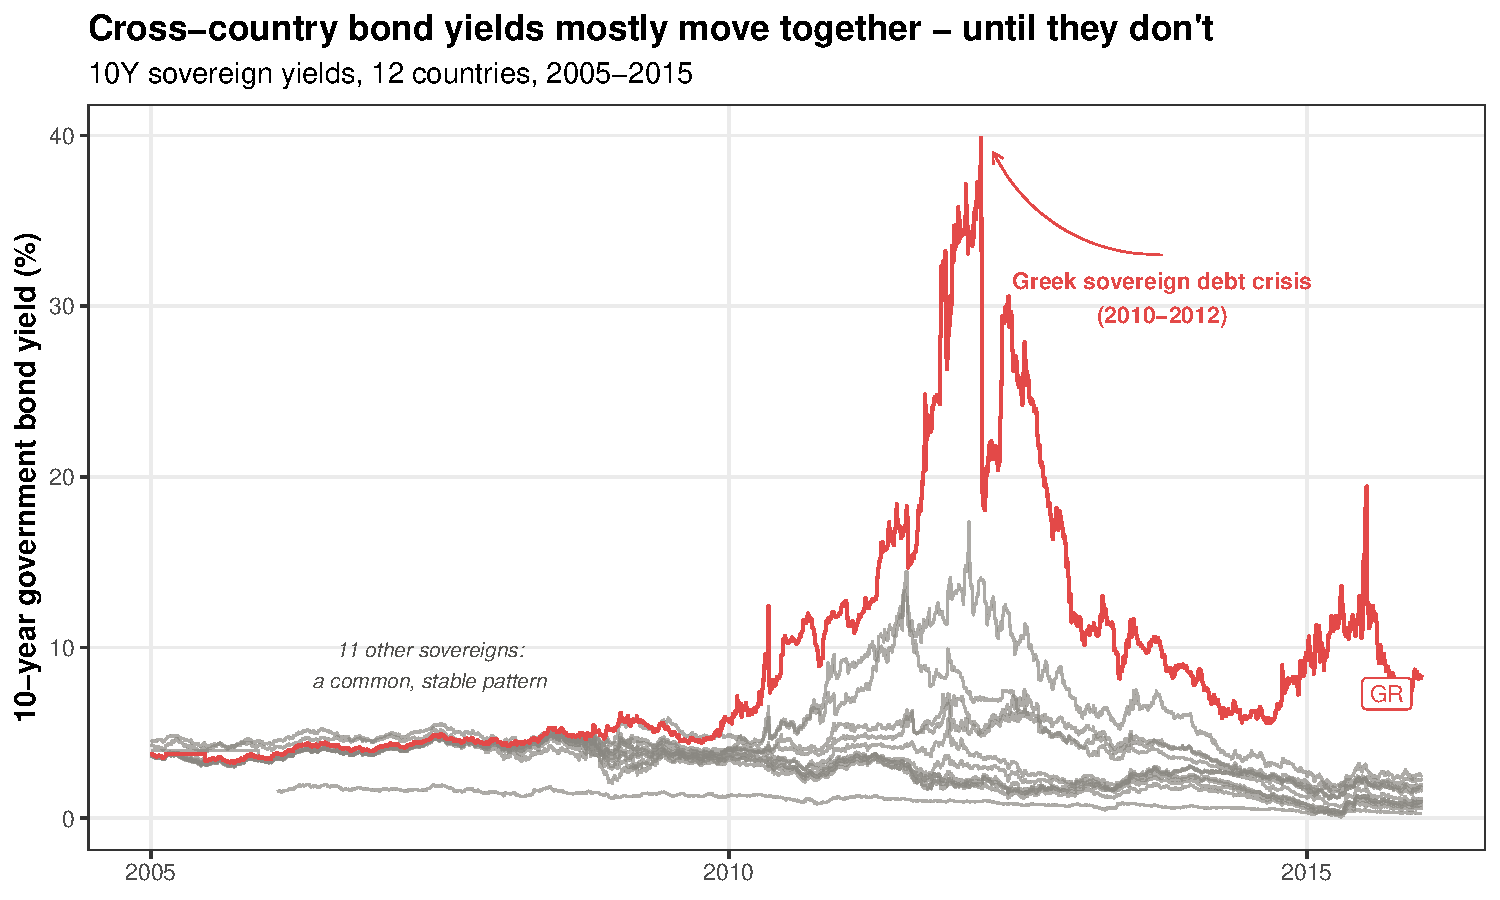
\includegraphics[width = \textwidth]{../../figures/rank_rsvddpd/motivating_bond_yields.pdf}

\end{frame}


\begin{frame}{Factor Models, but with outliers}
    \begin{itemize}
        \item The above data can be represented as a matrix.
        \item Rows represent time points, and columns represent countries.
        \item The underlying factors provide a low-rank signal to the matrix data.
    \end{itemize}

    \begin{equation*}
        \bb{X}_{n \times p} = \bb{L} + \bb{E},
    \end{equation*}
    \noindent where $\bb{L}$ is a low-rank matrix of rank $r$, and $\bb{E}$ is a noise matrix with
    \begin{equation*}
        E_{ij} \sim_{\text{IID}} (1-\epsilon) f + \epsilon k
    \end{equation*}
    \noindent where $f$ is the modelling density, and $k$ is the contamination density.

\end{frame}

\begin{frame}{Recommender Systems: Shilling Attacks}
    \begin{itemize}
        \item Recommendation systems are widely used in e-commerce platforms to recommend products to users.
        \item Collected data includes (user, item) pairs and corresponding ratings.
        \item Underlying factors reveal the preferences of users and the characteristics of items.
    \end{itemize}
    \vspace*{1em}
    \pause

    
\includegraphics[width = 0.49\textwidth]{../../figures/rank_rsvddpd/shilling-cnbc.png}
    
\includegraphics[width = 0.49\textwidth]{../../figures/rank_rsvddpd/shilling-paper.png}


    % \footnote{Manipulating Recommender Systems: A Survey of Poisoning Attacks and Countermeasures. Nguyen et al. (2024). \url{https://arxiv.org/pdf/2404.14942v1}}

    % \todo{Add articles on shilling attacks in recommender systems}
    % \todo{https://www.cnbc.com/2019/04/16/amazon-flooded-with-thousands-of-fake-reviews-report-claims.html}
    % \todo{https://www.rpubs.com/OlgaShiligin/503587}
\end{frame}


\begin{frame}{Recommender Systems: MovieLens Data}
    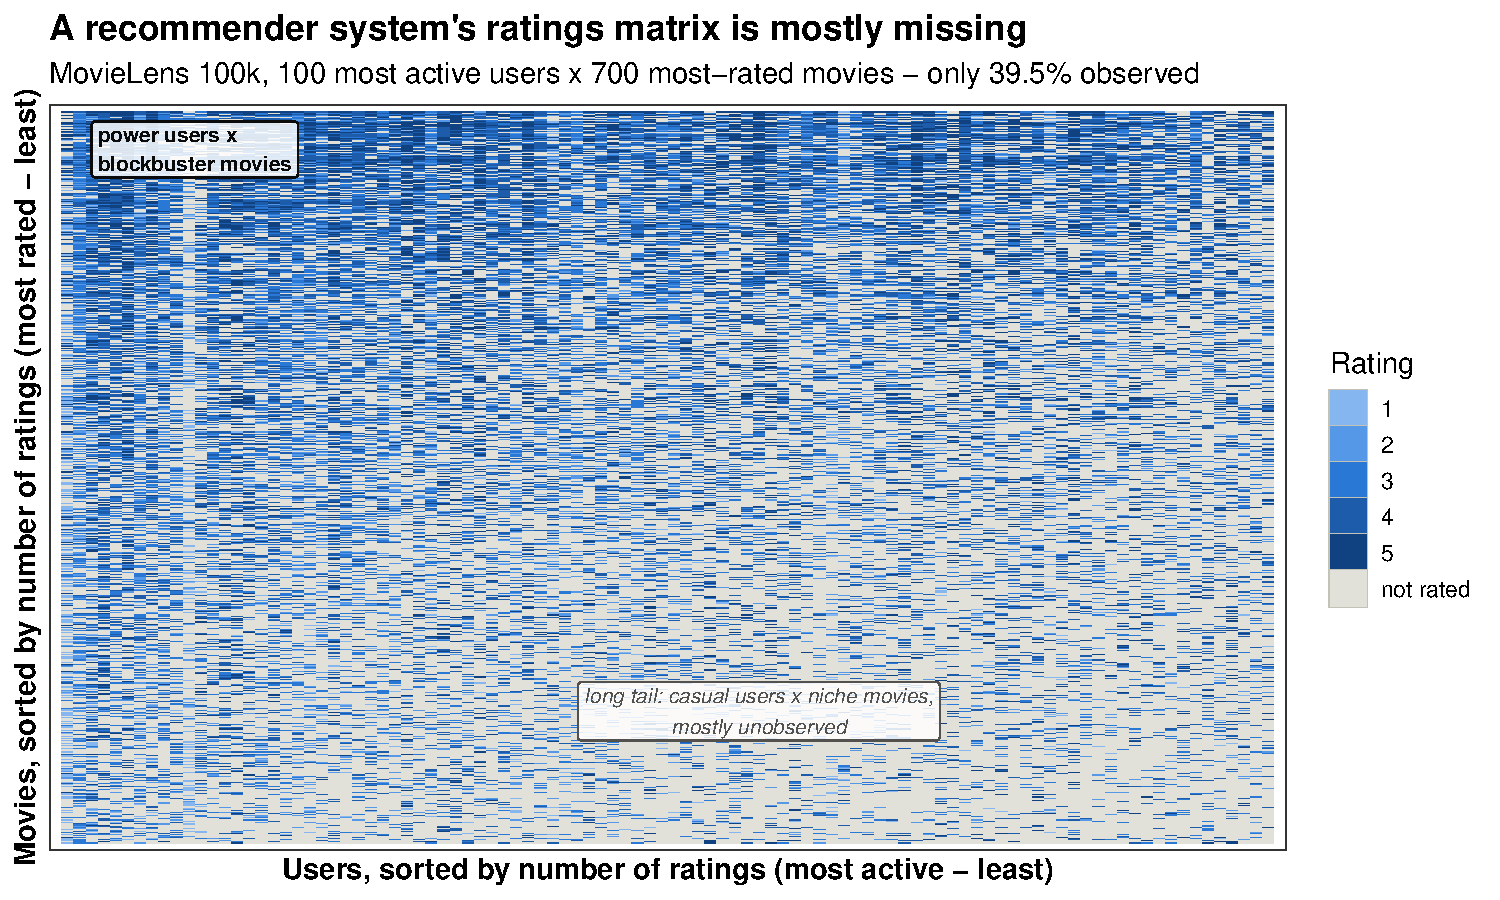
\includegraphics[width = \textwidth]{../../figures/rank_rsvddpd/motivating_reco_sparsity.pdf}
\end{frame}

\begin{frame}{Ubiquity of Matrix Decomposition}
    The $\bb{L} + \bb{E}$ decomposition arises across many different fields.
    \begin{enumerate}
        \item \emph{Background Modelling:} In video surveillance data, background is like low-rank slowing varying signal, and the noise (or sparse components) are like foregrounds~\cite{roy2024rsvddpd}.
        \item \emph{Gene Expression:} Gene expression matrices are typically partially completed, and outliers exist due to lack of precise measurements. The low-rank component provides underlying biological factors~\cite{linderman2022ALRA}.
    \end{enumerate}
\end{frame}



\thanksframe{Core Challenges}

\begin{frame}{Robust Singular Value Decomposition}
    \begin{itemize}
        \item The classical SVD is not robust to outliers.
        \item We need a robust SVD method to estimate the low-rank component $\bb{L}$.
    \end{itemize}

    \alert{\emph{Assume that the rank $r$ is known.}}

    \pause
    Then,
    \begin{equation*}
        X_{ij} = \sum_{k=1}^r U_{ik} D_{kk} V_{jk} + E_{ij} = \sum_{k=1}^r a_{ik} b_{jk} + E_{ij},
    \end{equation*}
    \pause
    \noindent Fix $j$, and get 
    \begin{equation*}
        (X_{\cdot j})_{n \times 1} = \bb{A}_{n \times r} (B_{j\cdot})_{r \times 1} + E_{\cdot j}
    \end{equation*}
    \noindent Assuming $\bb{A}$ is known, we can estimate each $(B_{j\cdot})$ by solving a \alert{robust} regression problem.
\end{frame}

\begin{frame}{Robust SVD: The Iterative Regression}
    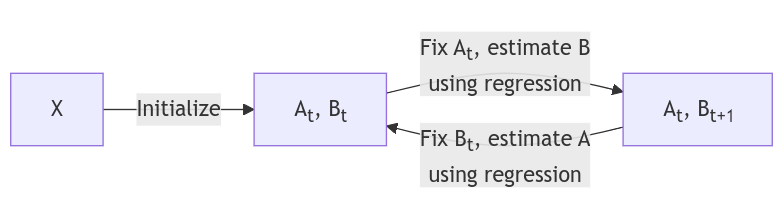
\includegraphics[width = \textwidth]{../../figures/thesis_slides/diagram.png}

    \begin{enumerate}
        \item Assume that rank $r$ is known.
        \item Initialize $\bb{A}_0 = \bb{A}$ and $\bb{B}_0 = \bb{B}$ using classical SVD (or random orthogonal matrices, scaled by the singular values).
        \item Given $A_{t}$, estimate $B_{t+1}$ by solving $p$ robust multiple linear regression problems.
        \item Given $B_{t+1}$, estimate $A_{t+1}$ by solving $n$ robust multiple linear regression problems.
        \item Repeat until convergence.
    \end{enumerate}
\end{frame}


\begin{frame}{What if $r$ is unknown?}

    \textbf{Naive Implementation}
    Since $r$ is also the number of true non-zero regression coefficients, we can use regression variable selection methods (e.g., LASSO, SCAD, Knockoffs, etc.)

    \pause
    \vspace*{1em}
    \textcolor{red}{\textbf{Problem:}} Selected variables may be different for different choices of $j = 1, \dots, p$ -- there is no single, shared $r$.

    \pause
    \vspace*{0.5em}
    \begin{center}
        \alert{Two broad strategies dominate the literature}:
    \end{center}
    \begin{enumerate}
        \item \textbf{Information criteria} -- penalize objective function $d(\cdot)$ analytically, in closed form.
        \item \textbf{Computational / resampling approaches} -- remove part of the data, refit, and measure prediction error on the held-out part.
    \end{enumerate}
\end{frame}

\begin{frame}{Approach 1: Information Criteria}
    \begin{equation*}
        C(r) = d(\bb{X}, \widehat{\bb{L}}_r) + r a(\hat{\sigma}) g(n, p).
    \end{equation*}
    \noindent The rank is estimated as $\widehat{r} = \argmin_r C(r)$, and $\widehat{\bb{L}}_r$ from the rank $r$ approximation from SVD, $a(\cdot)$ is an appropriate function, and $g(\cdot)$ is the penalty.

    \pause
    \begin{itemize}
        \item Examples: AIC \cite{akaike1973information}, BIC \cite{schwarz1978estimating}, and the panel-data criteria PC1--PC3, IC1--IC3 of \cite{bai2002determining}.
        \item A related family: hard/soft \alert{thresholding} of singular values \cite{shabalin2013reconstruction, gavish2014optimal, choi2017selecting, xu2021adaptive}.
        \pause
        \item[\textcolor{red}{$\times$}] \textbf{Fast, closed-form} -- but classical criteria is built on $\Vert \bb{X} - \widehat{\bb{L}}_r\Vert_F^2$: \alert{a single outlier can dominate this term} and derail the whole criterion, \emph{even if $\widehat{\bb{L}}_r$ itself comes from a robust SVD}.
    \end{itemize}    
\end{frame}

\begin{frame}{Approach 2: Computational Approach}
    \begin{itemize}
        \only<1>{\item \textbf{Cross-validation / resampling}: hold out a subset of entries (or rows/columns), refit a rank-$r$ approximation on the rest, and measure prediction error on the held-out part -- repeat over folds and choose $r$ minimizing the prediction error.}
        \only<2>{
            \item Wold-style (or speckled) \cite{wold1978crossvalidation}. The removal of entries happen at each cell / entry level.
        }
        \only<3>{
            \item Eastment--Krzanowski \cite{eastment1982crossvalidation}, Gabriel-style \cite{gabriel2002lebiplot}, and bi-cross-validation \cite{owen2009bi}. The removal of entries happen at each row / column / block levels.
        }
    \end{itemize}
    \only<2>{
        \begin{center}
            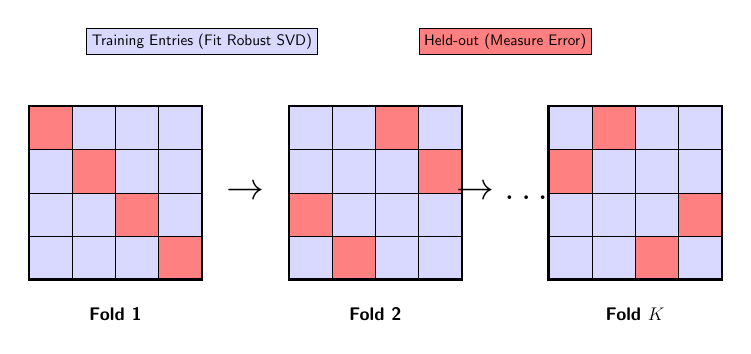
\begin{tikzpicture}[scale=0.55, transform shape]
            \tikzstyle{every node}=[font=\sffamily]
            
            % Legend
            \node[fill=blue!15, draw=black, minimum width=2.5cm, minimum height=0.6cm] at (4, 5.5) {Training Entries (Fit Robust SVD)};
            \node[fill=red!50, draw=black, minimum width=2.5cm, minimum height=0.6cm] at (11, 5.5) {Held-out (Measure Error)};
            
            % Matrix 1 (Fold 1)
            \begin{scope}[xshift=0cm]
                \fill[blue!15] (0,0) rectangle (4,4);
                % Held out cells
                \fill[red!50] (1,2) rectangle (2,3);
                \fill[red!50] (3,0) rectangle (4,1);
                \fill[red!50] (0,3) rectangle (1,4);
                \fill[red!50] (2,1) rectangle (3,2);
                \draw[step=1cm,black,very thin] (0,0) grid (4,4);
                \draw[thick] (0,0) rectangle (4,4);
                \node at (2, -0.8) {\large \textbf{Fold 1}};
            \end{scope}

            \node at (5, 2) {\Huge $\rightarrow$};

            % Matrix 2 (Fold 2)
            \begin{scope}[xshift=6cm]
                \fill[blue!15] (0,0) rectangle (4,4);
                % Held out cells
                \fill[red!50] (0,1) rectangle (1,2);
                \fill[red!50] (2,3) rectangle (3,4);
                \fill[red!50] (1,0) rectangle (2,1);
                \fill[red!50] (3,2) rectangle (4,3);
                \draw[step=1cm,black,very thin] (0,0) grid (4,4);
                \draw[thick] (0,0) rectangle (4,4);
                \node at (2, -0.8) {\large \textbf{Fold 2}};
            \end{scope}

            \node at (11, 2) {\Huge $\rightarrow \dots$};

            % Matrix 3 (Fold K)
            \begin{scope}[xshift=12cm]
                \fill[blue!15] (0,0) rectangle (4,4);
                % Held out cells
                \fill[red!50] (2,0) rectangle (3,1);
                \fill[red!50] (0,2) rectangle (1,3);
                \fill[red!50] (1,3) rectangle (2,4);
                \fill[red!50] (3,1) rectangle (4,2);
                \draw[step=1cm,black,very thin] (0,0) grid (4,4);
                \draw[thick] (0,0) rectangle (4,4);
                \node at (2, -0.8) {\large \textbf{Fold $K$}};
            \end{scope}
            \end{tikzpicture}
        \end{center}
    }

    \only<3>{
        \begin{center}
        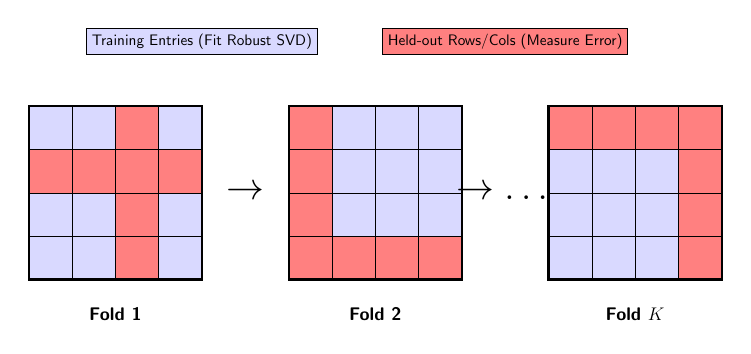
\begin{tikzpicture}[scale=0.55, transform shape]
        \tikzstyle{every node}=[font=\sffamily]
        
        % Legend
        \node[fill=blue!15, draw=black, minimum width=2.5cm, minimum height=0.6cm] at (4, 5.5) {Training Entries (Fit Robust SVD)};
        \node[fill=red!50, draw=black, minimum width=2.5cm, minimum height=0.6cm] at (11, 5.5) {Held-out Rows/Cols (Measure Error)};
        
        % Matrix 1 (Fold 1)
        \begin{scope}[xshift=0cm]
            \fill[blue!15] (0,0) rectangle (4,4);
            
            % Hold out Row 2 and Column 3
            \fill[red!50] (0,2) rectangle (4,3); % Row 2
            \fill[red!50] (2,0) rectangle (3,4); % Col 3
            
            \draw[step=1cm,black,very thin] (0,0) grid (4,4);
            \draw[thick] (0,0) rectangle (4,4);
            \node at (2, -0.8) {\large \textbf{Fold 1}};
        \end{scope}

        \node at (5, 2) {\Huge $\rightarrow$};

        % Matrix 2 (Fold 2)
        \begin{scope}[xshift=6cm]
            \fill[blue!15] (0,0) rectangle (4,4);
            
            % Hold out Row 4 and Column 1
            \fill[red!50] (0,0) rectangle (4,1); % Row 4
            \fill[red!50] (0,0) rectangle (1,4); % Col 1
            
            \draw[step=1cm,black,very thin] (0,0) grid (4,4);
            \draw[thick] (0,0) rectangle (4,4);
            \node at (2, -0.8) {\large \textbf{Fold 2}};
        \end{scope}

        \node at (11, 2) {\Huge $\rightarrow \dots$};

        % Matrix 3 (Fold K)
        \begin{scope}[xshift=12cm]
            \fill[blue!15] (0,0) rectangle (4,4);
            
            % Hold out Row 1 and Column 4
            \fill[red!50] (0,3) rectangle (4,4); % Row 1
            \fill[red!50] (3,0) rectangle (4,4); % Col 4
            
            \draw[step=1cm,black,very thin] (0,0) grid (4,4);
            \draw[thick] (0,0) rectangle (4,4);
            \node at (2, -0.8) {\large \textbf{Fold $K$}};
        \end{scope}
        \end{tikzpicture}
        \end{center}
    }
\end{frame}

\begin{frame}{Cross-validation Challenges}
    \begin{itemize}
        \item Using classical SVD leads to non-robust selection of rank.
        \item Can be robustified by swapping in a robust SVD at every fold \cite{alarcon2022cv} $\ldots$
        \item[\textcolor{red}{$\times$}] $\ldots$ \alert{but this is computationally prohibitive}:
        \begin{itemize}
            \item Gabriel-style CV on a modest $50 \times 40$ matrix needs $\approx 2000$ SVDs.
            \item At $\approx 1$ second per robust SVD, rank estimation alone takes $\approx 33$ minutes.
        \end{itemize}
        \pause
        \item One idea is to perform one full-rank (i.e., upto $\min(n,p)$) $\widehat{\bb{X}}$ from a single robust SVD of $\bb{X}$, which replaces outliers with reasonable predictions. Then apply cross-validation with classical SVD on $\widehat{\bb{X}}$, as it is free of outliers.
    \end{itemize}
\end{frame}



\begin{frame}{Other Approaches}
    \begin{itemize}
        \item \textbf{The ``Elbow'' method} \cite{thorndike1953elbow}: eyeball the scree plot of singular values for a visible drop. Simple, but subjective, and ill-defined under contamination.
        \item \textbf{Bayesian model averaging} over the rank and the SVD components \cite{hoff2007model}.
        \item \textbf{Spectral regularization} / nuclear-norm penalization with soft-imputation \cite{mazumder2010spectral}.
        \pause
        \item[\textcolor{red}{$\times$}] None of these were designed with robustness to outliers in mind.
    \end{itemize}
\end{frame}

\thanksframe{Divergence Information Criterion for Matrix Rank}

\begin{frame}{Robust SVD Objective function}
    \small
    \begin{definition}
        \cite{basu1998dpd} defined the \emph{density power divergence} between two probability densities $f$ and $g$ as 
        \begin{equation*}
            d_\alpha(f, g) = \int f^{1+\alpha} - \left(1 + \frac{1}{\alpha} \right)\int f^\alpha g + \frac{1}{\alpha}\int g^\alpha,
        \end{equation*}        
        \noindent where $\alpha > 0$ is the robustness parameter.
    \end{definition}
    \pause

    \noindent In the Robust SVD context, let $f$ be the model density, $\theta = (\bb{U}, \bb{D}, \bb{V}, \sigma^2)$ be parameters from SVD. Then,
    \begin{equation*}
        H_\alpha(\bb{\theta}) = \frac{1}{\sigma^\alpha} \left[ \int f^{1+\alpha} - \left( 1 + \frac{1}{\alpha} \right) \frac{1}{np}\sum_{i=1}^n\sum_{j=1}^p f^\alpha\left( \frac{X_{ij} - (\bb{UDV}\tr)_{ij}}{\sigma} \right)\right].
    \end{equation*} 
\end{frame}


\begin{frame}{Derivation}
    \small
    \only<1->{DIC is simply unbiased estimate of $Q_\alpha(\widehat{\theta})$, where
    \begin{equation*}
        Q_\alpha(\theta) = \mathbb{E}_{\bb{X}}(H_\alpha(\theta)), \text{ for all } \theta \in \Theta
    \end{equation*}}
    \vspace*{-1em}
    \begin{align*}
        \only<2->{Q_\alpha(\bbhat{U}, \bbhat{D}, \bbhat{V}, \hat{\sigma}^2) 
        & = \E\left( Q_\alpha(\bbhat{U}, \bbhat{D}, \bb{V}, \hat{\sigma}^2) \mid \bb{V} = \bbhat{V} \right)}\\
        & \only<3->{= \E\left( \E\left( H_\alpha(\bbhat{U}, \bbhat{D}) + \dfrac{1}{n}\hat{\sigma}^{-\alpha} \trace(\bb{V}\tr \bb{V}) \dfrac{C_{2\alpha}}{C_\alpha} \right) \mid \bb{V} = \bbhat{V} \right)}\\
        & \only<4->{= \E\left( H_\alpha(\hat{\theta}) + \dfrac{r}{n}\hat{\sigma}^{-\alpha}\dfrac{C_{2\alpha}}{C_\alpha} \right)}\\
        & \only<5->{= \E\left( H_\alpha(\hat{\theta}) + \dfrac{r}{p}\hat{\sigma}^{-\alpha}\dfrac{C_{2\alpha}}{C_\alpha} \right), \text{ by symmetry}}\\
        & \only<6->{= \E\left( \underbrace{ H_\alpha(\hat{\theta}) + r \dfrac{(1/n+1/p)}{2}\hat{\sigma}^{-\alpha}\dfrac{C_{2\alpha}}{C_\alpha}}_{\blue{\mathrm{DICMR}_{\alpha,1}(r)}} \right)}
    \end{align*}
\end{frame}

\begin{frame}{Assumptions}
    \begin{enumerate}
        \item The model density $f$ is symmetric about $0$, decreasing in $\vert x\vert$ and is differentiable in $\vert x\vert$.
        \item $\sup_{x \in \mathbb{R}} \max\left\{ \vert f^\alpha(x)\nabla \log(f(x)) \vert, \vert x f^\alpha(x)\nabla \log(f(x)) \vert \right\} < \infty$.
        \item True noise variance $\sigma^2 \asymp (np)^{-1/2}$. 
        \item Estimated noise variance $\hat{\sigma}^2$ lies between $[\sigma^2_{\min}, \sigma^2_{\max}]$ with $\sigma^2_{\min} \asymp (np)^{-1/2}$ and $\sigma^2_{\max} \asymp 1$. 
    \end{enumerate}
    \pause

    \vspace*{1em}
    Standard $f$ ensures (1) and (2) holds, e.g., Gaussian, $t$, logistic, etc.\\

    \vspace*{0.5em}
    Assumption 3 is \alert{necessary}, \cite{shabalin2013reconstruction} showed with any larger error variance, the singular values (or their functions) cannot be consistently estimated.
\end{frame}

\begin{frame}{Underestimation Probability}
    \small
    \begin{theorem}[Simplified]
        Consider a criterion of the form
        \begin{equation*}
            C_\alpha(r) = H_\alpha(\hat{\theta}) + r \gamma_{n,p} \widehat{\sigma}^{-\alpha},
        \end{equation*}
        \noindent where $\gamma_{n,p} > 0$ is a sequence of positive constants. Suppose $r < r^\ast$, the true rank, and $\sigma^\ast_{r,\alpha} \geq \sigma(1 + O(1)), \gamma_{n,p} = o(1)$. Then,
        \begin{equation*}
            \prob(C_\alpha(r) \leq C_\alpha(r^\ast))
            \leq C_1 \exp\left( -npC_2 + C_3 (n+p+1)r^\ast\log(np) \right),
        \end{equation*}
        \noindent where $C_1, C_2$ and $C_3$ are some generic constants independent of $n$ and $p$.
    \end{theorem}
\end{frame}

\begin{frame}{Overestimation Probability}
    \small
    \begin{theorem}[Simplified]
        Consider a criterion of the form
        \begin{equation*}
            C_\alpha(r) = H_\alpha(\hat{\theta}) + r \gamma_{n,p} \widehat{\sigma}^{-\alpha},
        \end{equation*}
        \noindent where $\gamma_{n,p} > 0$ is a sequence of positive constants. Pick any $r \in (r^\ast, r_{\max}]$, where $r^\ast$ is the true rank. Then, 
        \begin{equation*}
            \prob(C_\alpha(r) \leq C_\alpha(r^\ast)) \leq \max\{ B(r_{\max}), B(r^\ast) \},
        \end{equation*}
        \noindent where 
        \begin{equation*}
            B(r) = C_5 \exp\left( -npC_6 \gamma_{n,p}^2 + C_7 ((n+p+1)r+1)\log(np) \right)
        \end{equation*}
        \noindent for some appropriate positive constants $C_5, C_6, C_7$ free of $n, p$ and $r$, depending on the true rank $r^\ast$. 
    \end{theorem}
\end{frame}

\begin{frame}{The Second variant of DICMR}
    \begin{center}
    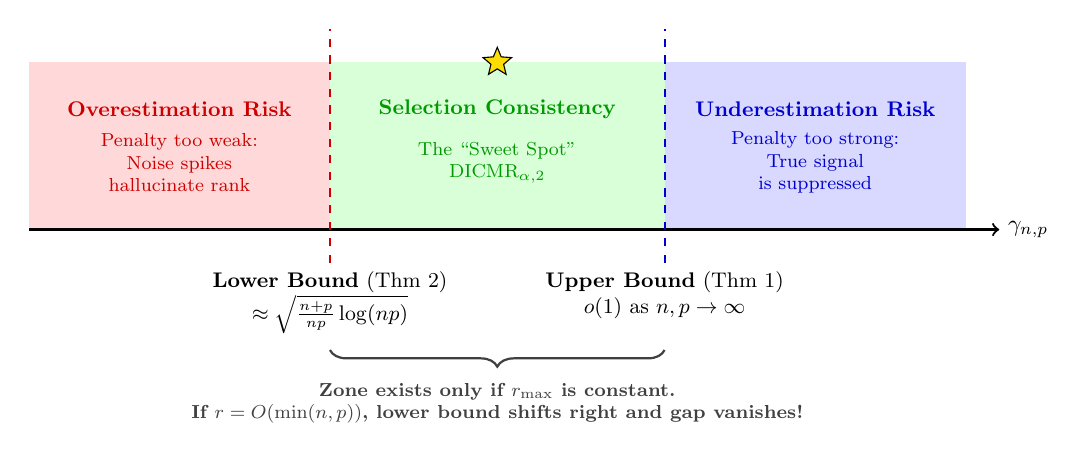
\begin{tikzpicture}[scale=0.85, transform shape]
        % Define colors for the zones
        \colorlet{overcolor}{red!15}
        \colorlet{undercolor}{blue!15}
        \colorlet{safecolor}{green!15}

        % 1. Overestimation Region (Left)
        \fill[overcolor] (0,0) rectangle (4.5, 2.5);
        \node[red!80!black, align=center, font=\small\bfseries] at (2.25, 1.8) {Overestimation Risk};
        \node[red!80!black, align=center, font=\footnotesize] at (2.25, 1.0) {Penalty too weak:\\Noise spikes \\ hallucinate rank};

        % 2. Selection Consistency Region (Middle)
        \fill[safecolor] (4.5,0) rectangle (9.5, 2.5);
        \node[green!60!black, align=center, font=\small\bfseries] at (7, 1.8) {Selection Consistency};
        \node[green!60!black, align=center, font=\footnotesize] at (7, 1.0) {The ``Sweet Spot''\\$\text{DICMR}_{\alpha,2}$};

        % 3. Underestimation Region (Right)
        \fill[undercolor] (9.5,0) rectangle (14, 2.5);
        \node[blue!80!black, align=center, font=\small\bfseries] at (11.75, 1.8) {Underestimation Risk};
        \node[blue!80!black, align=center, font=\footnotesize] at (11.75, 1.0) {Penalty too strong:\\True signal \\ is suppressed};

        % The Axis
        \draw[->, thick] (0,0) -- (14.5,0) node[right, font=\bfseries] {$\gamma_{n,p}$};

        % Lower Bound Boundary (Theorem 2)
        \draw[thick, dashed, red!80!black] (4.5,-0.5) -- (4.5,3);
        \node[below, align=center, font=\small] at (4.5, -0.5) {\textbf{Lower Bound} (Thm 2) \\ $\approx \sqrt{\frac{n+p}{np}\log(np)}$};

        % Upper Bound Boundary (Theorem 1)
        \draw[thick, dashed, blue!80!black] (9.5,-0.5) -- (9.5,3);
        \node[below, align=center, font=\small] at (9.5, -0.5) {\textbf{Upper Bound} (Thm 1) \\ $o(1)$ as $n,p \to \infty$};

        % Explanatory Brace for the r_max limitation
        \draw[decorate,decoration={brace,amplitude=6pt,mirror}, xshift=0pt, yshift=-1.8cm, thick, darkgray]
        (4.5,0) -- (9.5,0) node [midway, yshift=-0.8cm, align=center, font=\footnotesize\bfseries, darkgray] {
            Zone exists only if $r_{\max}$ is constant. \\ If $r = O(\min(n,p))$, lower bound shifts right and gap vanishes!
        };
        
        % DICMR star
        \node[star, star points=5, star point ratio=2.25, fill=yellow!80!orange, draw=black, inner sep=2pt] at (7, 2.5) {};

    \end{tikzpicture}
    \end{center}

    \pause
    \begin{equation*}
        \text{DICMR}_{\alpha,2}(r) := H_{r,\alpha}(\bbhat{\theta}_{r,\alpha}) + \dfrac{r \sqrt{(n+p) \log(np)}}{2\sqrt{np}} \widehat{\sigma}_{r,\alpha}^{-\alpha} C^f_{2\alpha}/C^f_{\alpha}
    \end{equation*}
\end{frame}


\begin{frame}{B-Robustness}
    \begin{theorem}
        Consider a criterion of the form
        \begin{equation*}
            C_\alpha(r) = H_\alpha^{(r)}(\hat{\theta}) + r \gamma_{n,p} \widehat{\sigma}^{-\alpha},
        \end{equation*}
        \noindent where $\gamma_{n,p} > 0$ is a sequence of positive constants. The model selection criterion $C_\alpha(r)$ is first-order B-robust for any $\alpha > 0$, provided that the corresponding $\mathrm{rSVDdpd}$ estimator (i.e., the iterative method to estimate $\hat{\theta}$ by minimizing DPD) is B-robust, and $\gamma_{n,p} = O(1)$.
    \end{theorem}
\end{frame}



\thanksframe{Experimental Results}


\begin{frame}{Simulation Settings}
    \begin{itemize}
        \item Random orthogonal matrices as left (and right) singular vectors.
        \item Two settings: (i) First $r$ singular values are $1$, rest are $0$. (ii) The singular values are $2, 1 + (r-2)/(r-1), \dots, 1$, and rest are $0$.
        \item Noise entries are i.i.d. normal with mean zero and variance $\sigma_e^2 = \mathbb{E}(\Vert \bb{L}\Vert_F^2) / (np \times \text{SNR})$.
        \item SNR levels are $2, 4$ and $10$. Randomly chosen $5\%, 10\%$ or $20\%$ entries are contaminated with a value twice of the maximum.
    \end{itemize}
\end{frame}

\begin{frame}{Simulation Results}
    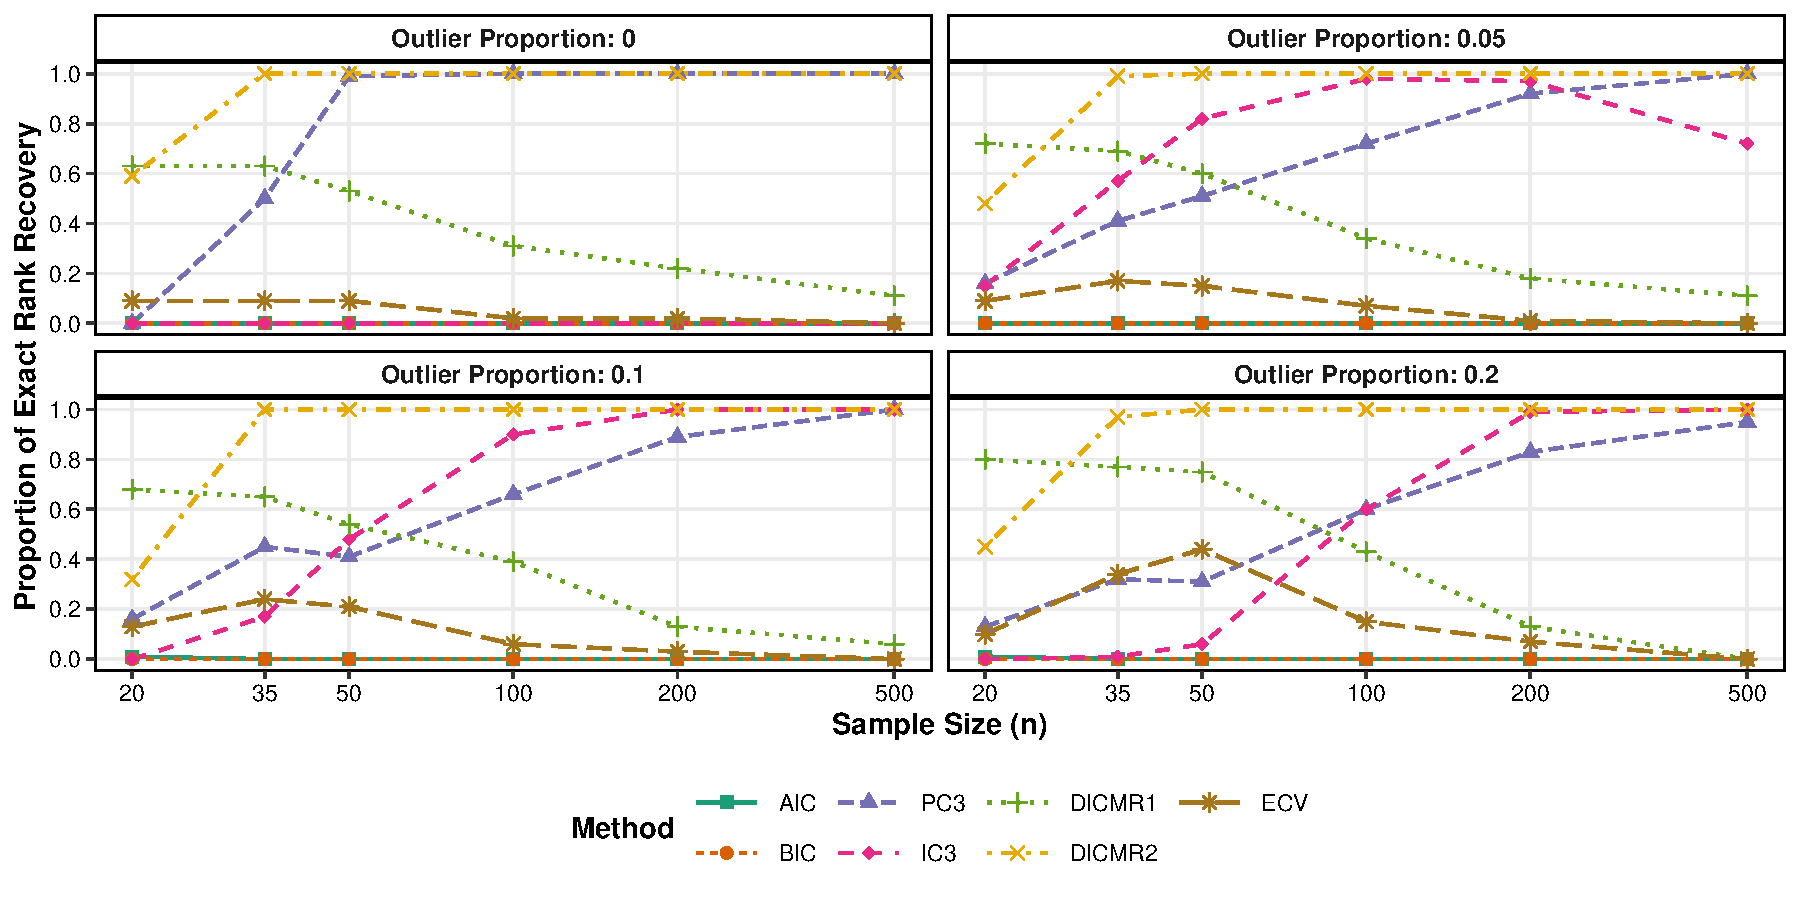
\includegraphics[width = \textwidth]{../../figures/rank_rsvddpd/exact_rank_recovery_eigsame.pdf}
\end{frame}

\begin{frame}{Simulation Results}
    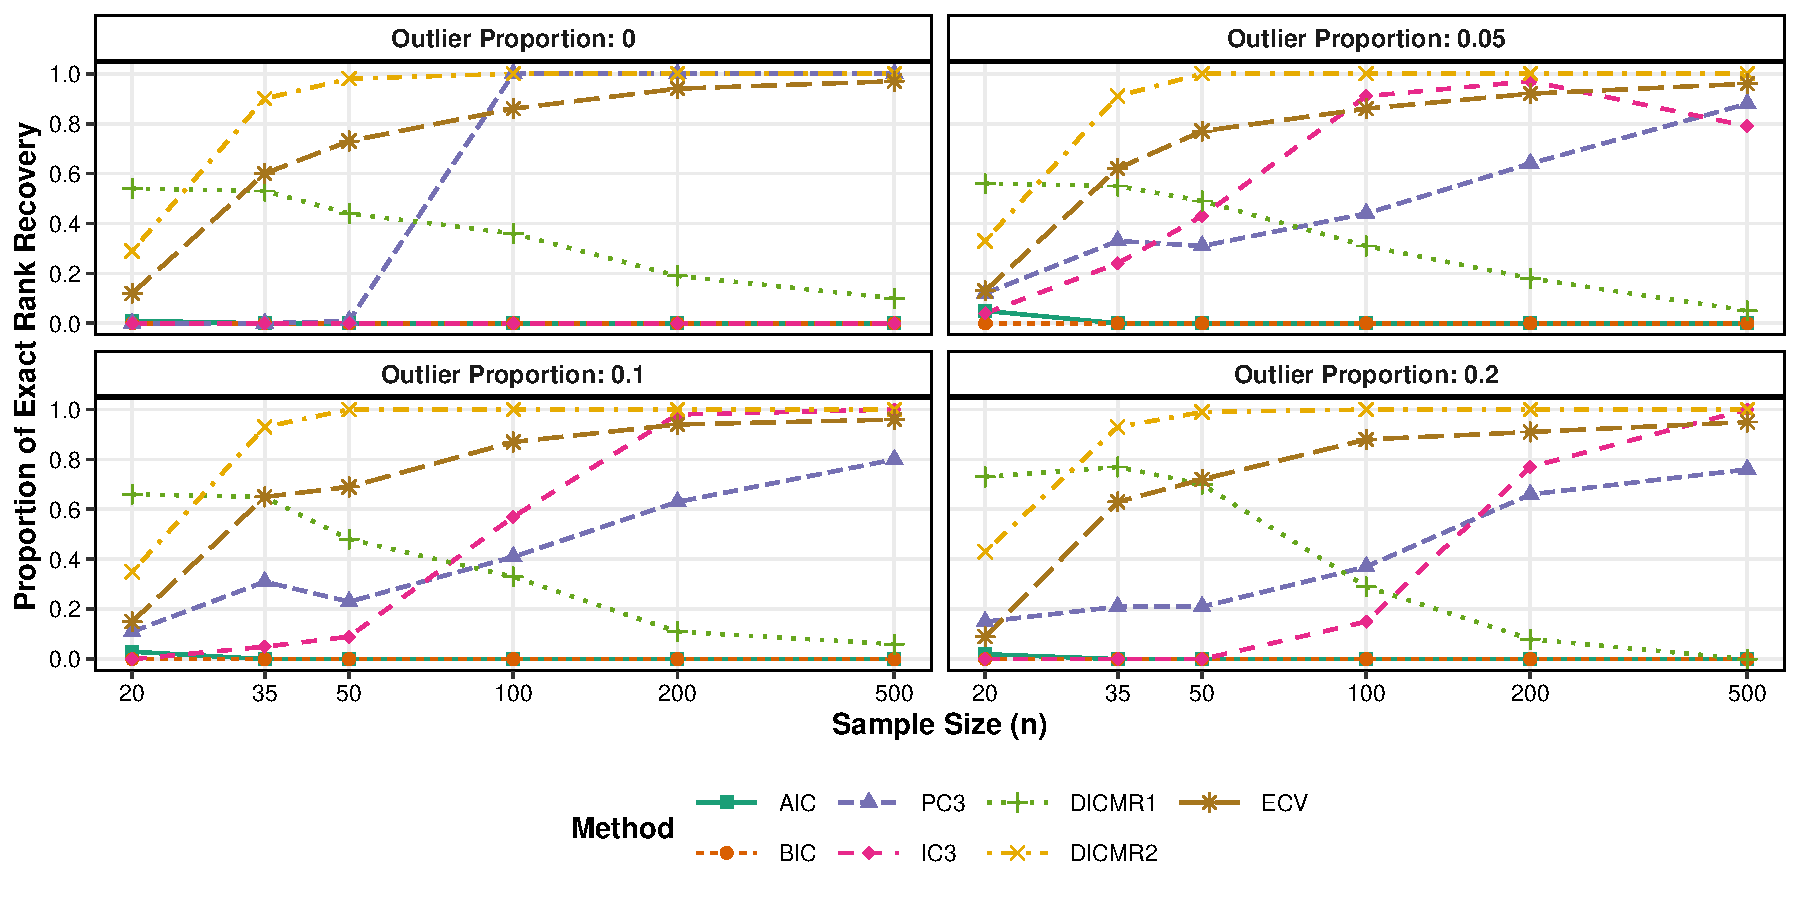
\includegraphics[width = \textwidth]{../../figures/rank_rsvddpd/exact_rank_recovery_eigdec.pdf}
\end{frame}

\begin{frame}{Finite-Sample Tuning}
    \small
    \begin{itemize}
        \item \textbf{Generalized Criterion:} Asymptotic consistency holds for a family of criteria scaled by a constant $c > 0$:
        \begin{equation*}
            \tilde{C}_{\alpha}(r) = H_{r,\alpha}(\bbhat{\theta}_{r,\alpha}) + c \cdot r \hat{\sigma}_{r,\alpha}^{-\alpha} \frac{\sqrt{(n+p)\log(np)}}{\sqrt{np}}
        \end{equation*}
        \item \textbf{The Challenge:} For finite $n$ and $p$, the penalty requires careful tuning. 
        \begin{itemize}
            \item $c$ too small $\implies$ Penalty too weak (Overestimation)
            \item $c$ too large $\implies$ Penalty too aggressive (Underestimation)
        \end{itemize}
    \end{itemize}
\end{frame}

\begin{frame}{Finite-Sample Tuning: The Plateau Heuristic}
    \textbf{The Plateau Heuristic:} Evaluate optimal rank $r(c)$ over a grid of $c$. The true rank is highly stable against perturbations, corresponding to the \textbf{widest flat region}~\cite{hallin2007determining}.

    \begin{center}
    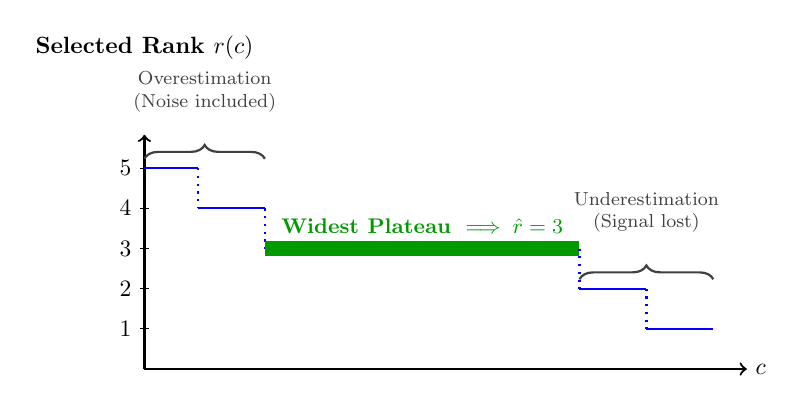
\begin{tikzpicture}[scale=0.85, transform shape]
        % Axes
        \draw[->, thick] (0,0) -- (9,0) node[right, font=\bfseries] {$c$};
        \draw[->, thick] (0,0) -- (0,3.5) node[above, font=\bfseries, yshift=1cm] {Selected Rank $r(c)$};

        % Ticks
        \foreach \y in {1,2,3,4,5} \draw (2pt,\y*0.6) -- (-2pt,\y*0.6) node[left] {$\y$};
        
        % The Step Function Lines
        \draw[thick, blue] (0, 3.0) -- (0.8, 3.0);
        \draw[dotted, thick, blue] (0.8, 3.0) -- (0.8, 2.4);
        
        \draw[thick, blue] (0.8, 2.4) -- (1.8, 2.4);
        \draw[dotted, thick, blue] (1.8, 2.4) -- (1.8, 1.8);
        
        % The Plateau (Highlighted)
        \draw[line width=1.8mm, green!60!black] (1.8, 1.8) -- (6.5, 1.8);
        \node[above, green!60!black, font=\small\bfseries] at (4.15, 1.9) {Widest Plateau $\implies \hat{r} = 3$};
        
        \draw[dotted, thick, blue] (6.5, 1.8) -- (6.5, 1.2);
        
        \draw[thick, blue] (6.5, 1.2) -- (7.5, 1.2);
        \draw[dotted, thick, blue] (7.5, 1.2) -- (7.5, 0.6);
        
        \draw[thick, blue] (7.5, 0.6) -- (8.5, 0.6);

        % Annotations with Braces
        \draw[decorate,decoration={brace,amplitude=5pt},yshift=4pt, thick, darkgray] (0, 3.0) -- (1.8, 3.0) node [midway, yshift=0.5cm, font=\footnotesize, align=center, yshift = 0.5cm] {Overestimation \\ (Noise included)};
        
        \draw[decorate,decoration={brace,amplitude=5pt},yshift=4pt, thick, darkgray] (6.5, 1.2) -- (8.5, 1.2) node [midway, yshift=0.5cm, font=\footnotesize, align=center, yshift = 0.5cm] {Underestimation \\ (Signal lost)};
        
    \end{tikzpicture}
    \end{center}
\end{frame}


\begin{frame}{Bond Yield Data: Classical Criteria Find Nothing}
    \small
    \begin{itemize}
        \item Panel of 10Y sovereign yields, 12 countries.
        \item Split into a calm window (2005--2009) and a window spanning the 2010--2012 Greek crisis (2005--2015).
    \end{itemize}

    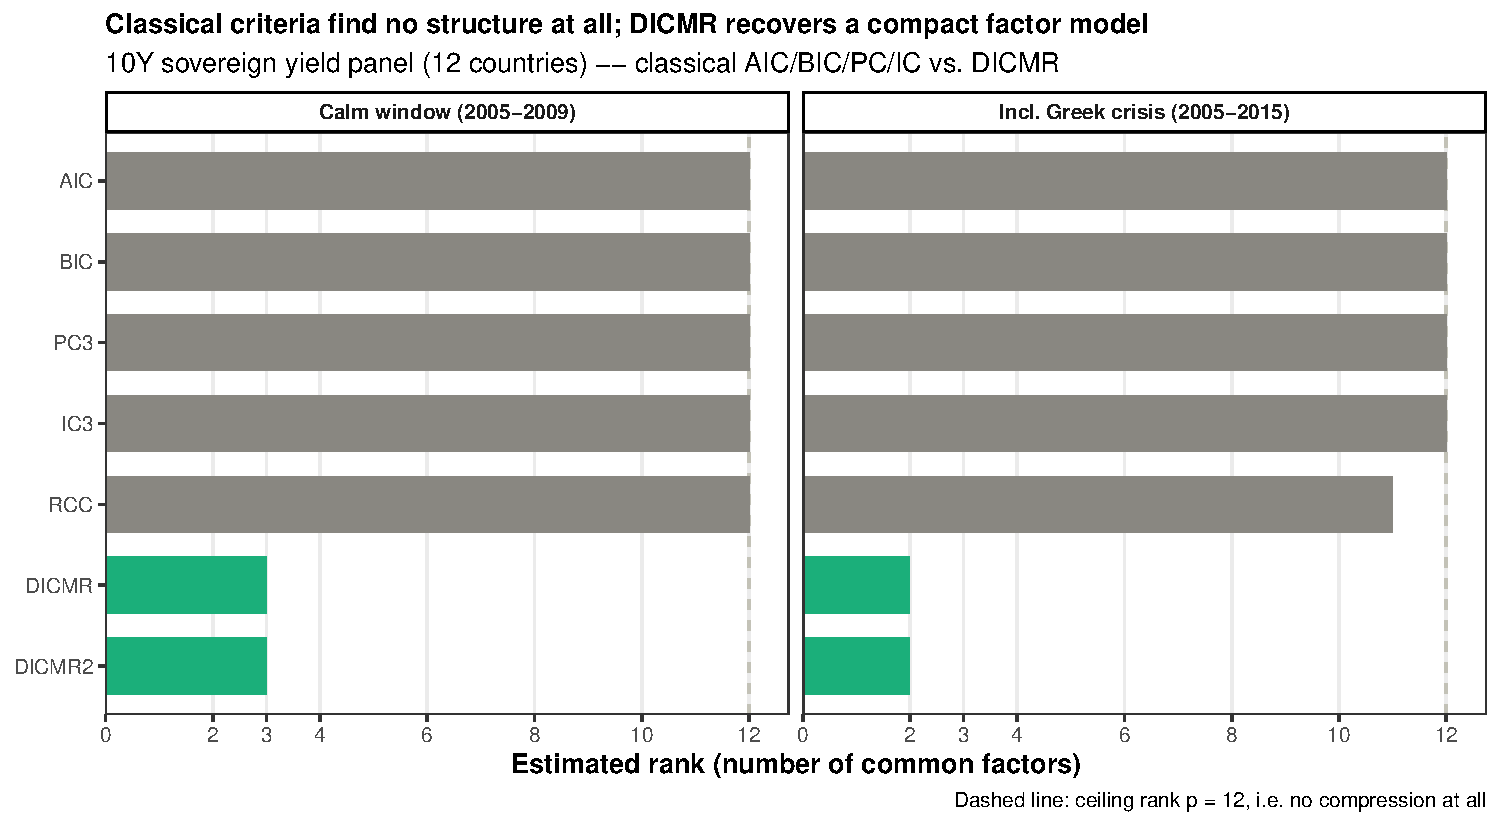
\includegraphics[width = 0.9\textwidth]{../../figures/rank_rsvddpd/results_bond_yield_rank.pdf}
\end{frame}

\begin{frame}{Bond Yield Data: What This Means}
    \begin{itemize}
        \item Every classical criterion picks $\widehat{r} = p = 12$ in \alert{both} windows: with only $12$ countries but thousands of trading days ($n \gg p$), their penalty is too weak to ever compress -- they treat every country as its own factor.
        \item DICMR / DICMR$_2$ instead recover a compact structure in both regimes: rank $3$ in the calm window, rank $2$ once the Greek crisis is included -- consistent with the textbook level/slope/curvature factor structure of yield curves. (\emph{e.g., Inflation, Central Bank Policy, Economic Activity, etc.})
    \end{itemize}
\end{frame}

\begin{frame}{Gene Expression: Why It Matters}
    \small
    \begin{itemize}
        \item RNA-sequencing data: rows are patient samples, columns are genes -- a handful of shared biological factors should drive a low-rank signal.
        \item Sequencing is costly, and combining multiple studies creates \alert{block-missing} patterns (some patients profiled on all genes, some genes profiled on all patients) -- a genuine matrix completion problem, not just random missingness.
        \item TCGA PAN-Cancer RNA-seq dataset \cite{gene_expression_data}: $801$ patient samples $\times$ $20{,}531$ genes, spanning $5$ cancer types, log2-normalized.
    \end{itemize}

    \begin{center}
        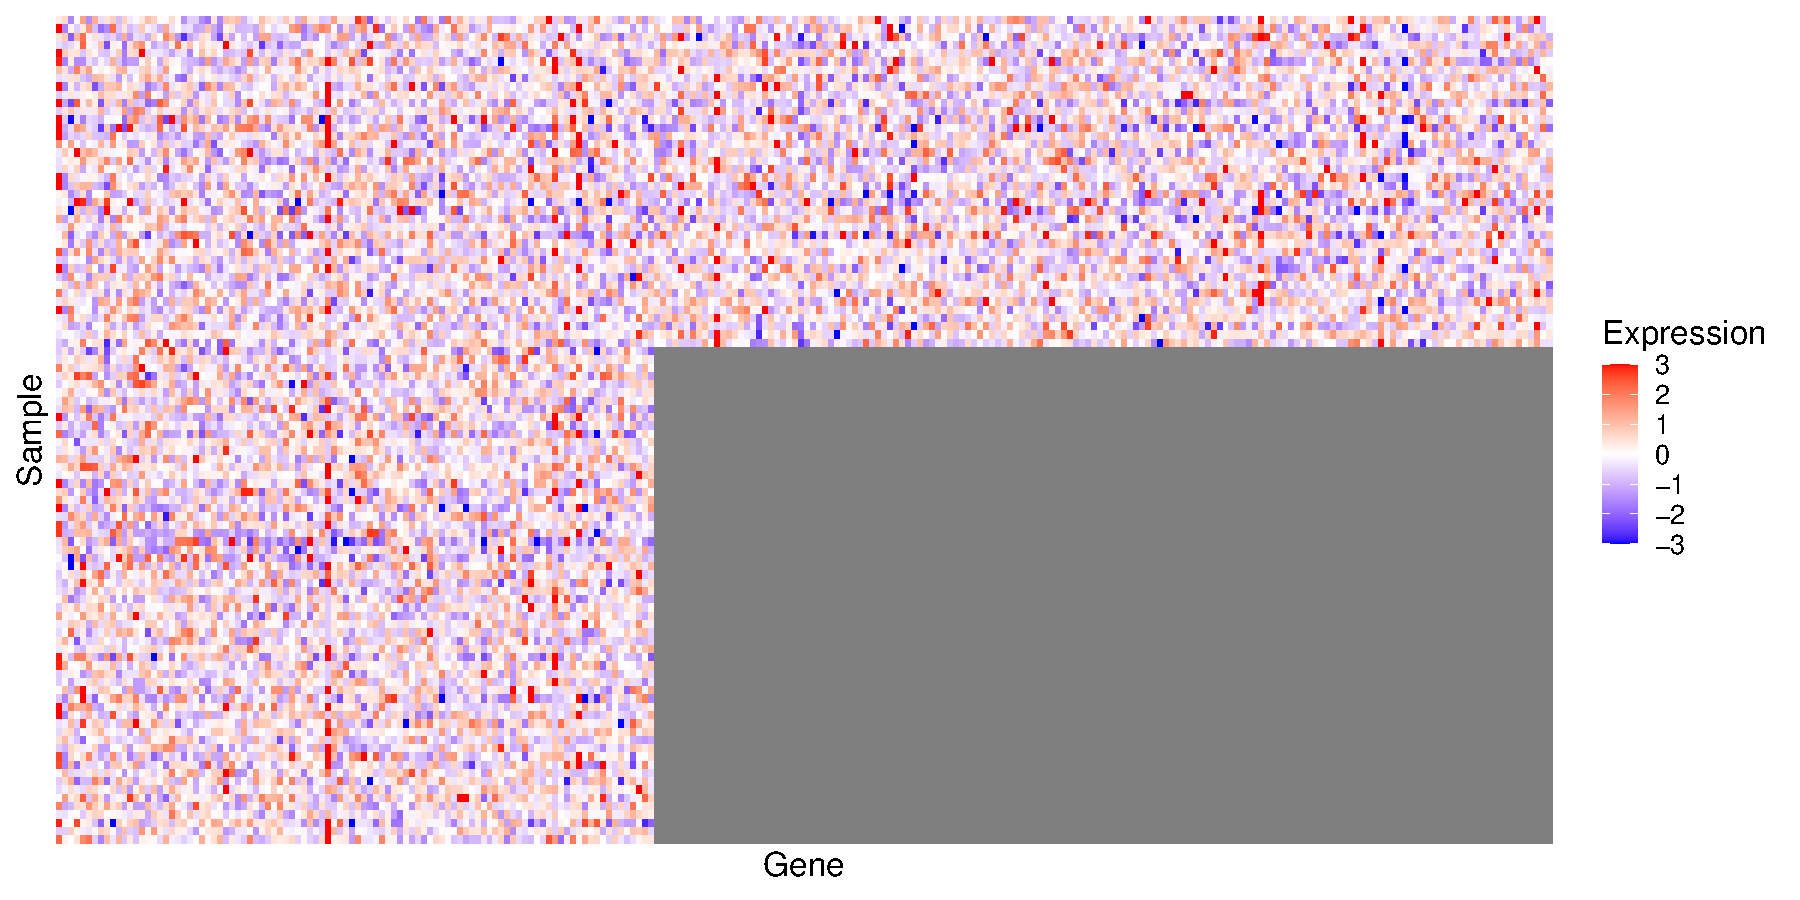
\includegraphics[width = 0.65\textwidth]{../../figures/rank_rsvddpd/gene_matrix_masked_data.pdf}
    \end{center}
\end{frame}

\begin{frame}{Gene Expression: Completions Compared}
    \small
    \begin{itemize}
        \item Train on a random $100 \times 2000$ block $\bb{Z}_{11}$; predict the held-out block $\bb{X}_{22}$ (below the dashed line) via $\bbhat{X}_{22} = \bb{X}_{21} [\bbhat{L}_{r,\alpha}]_{11}^{+} \bb{X}_{12}$.
        \item Several specialized methods collapse the held-out block to a near-constant value or show streaky artifacts; classical SVD and rSVDdpd stay coherent with the observed pattern.
    \end{itemize}

    \begin{center}
    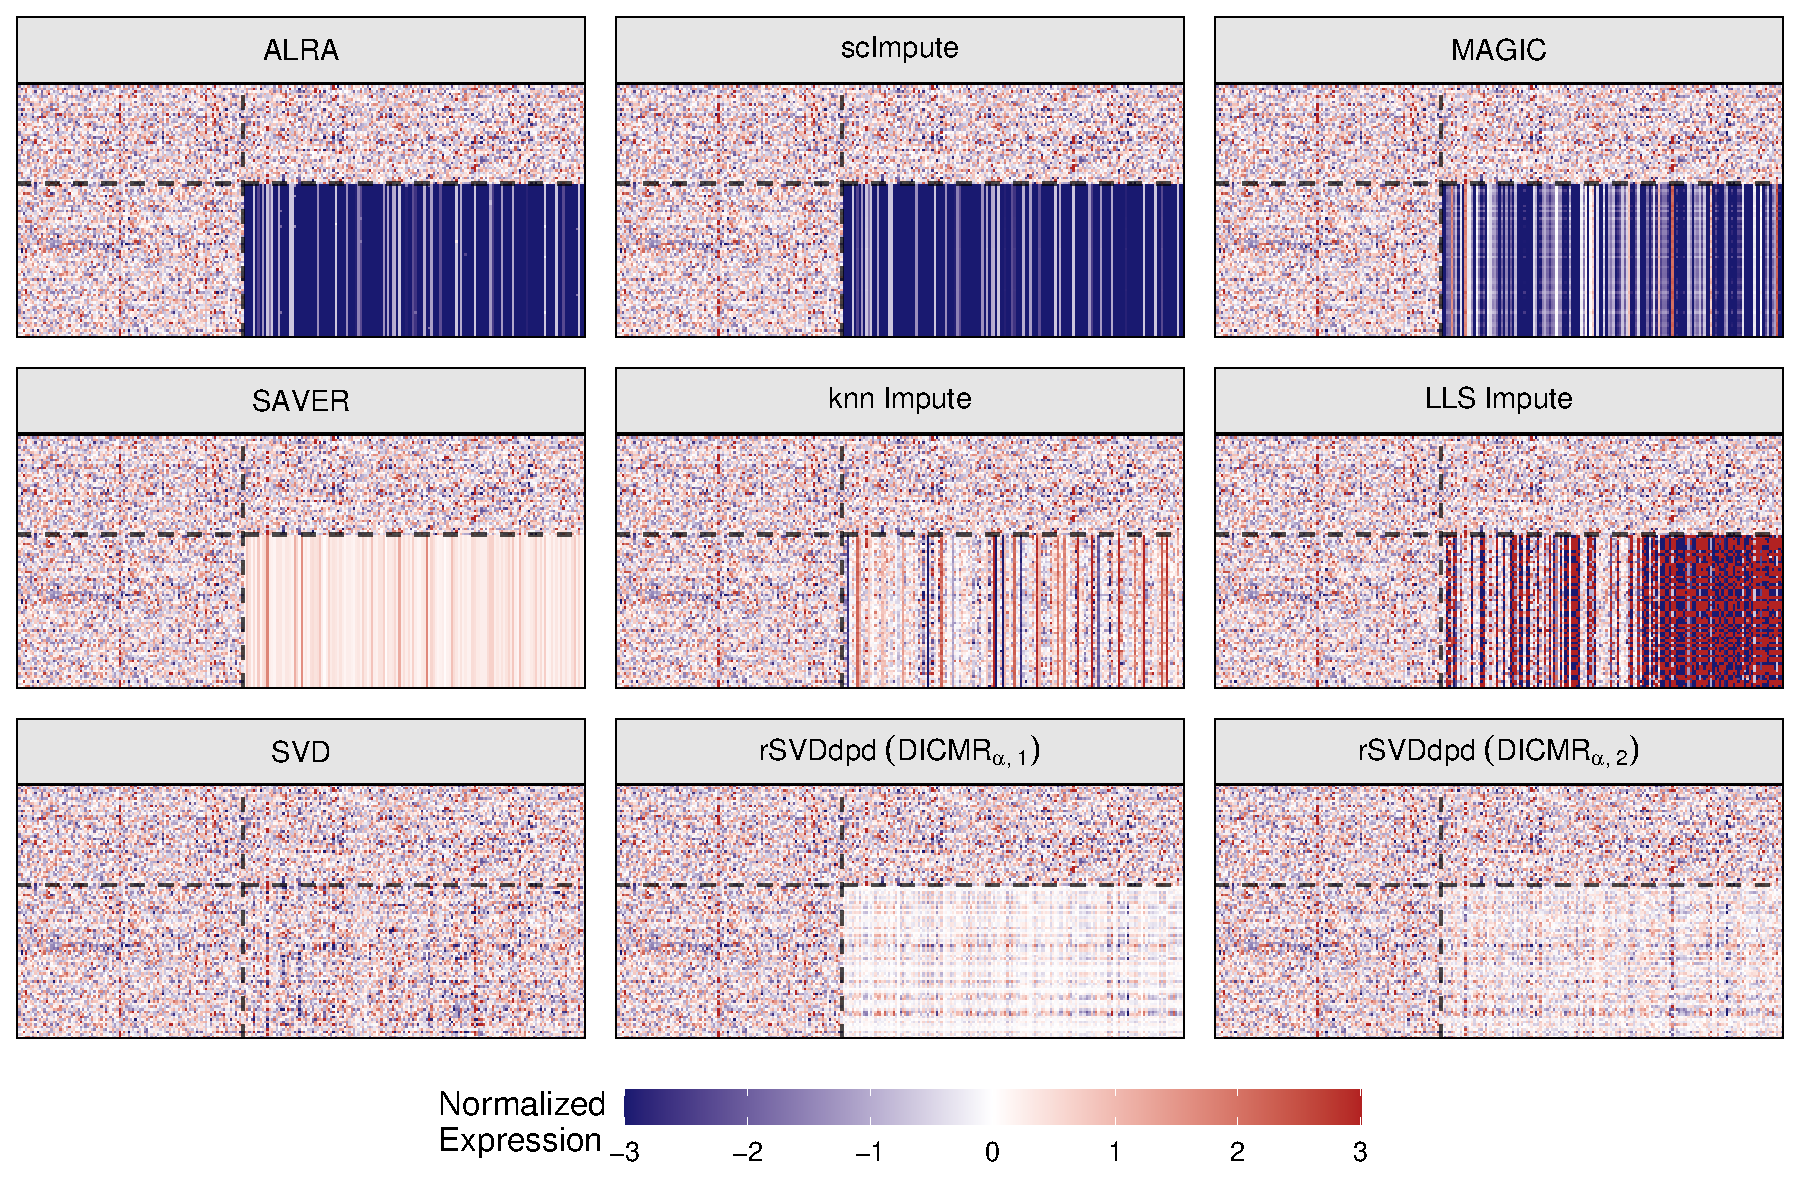
\includegraphics[width = 0.77\textwidth]{../../figures/rank_rsvddpd/gene_matrix_methods_completion.pdf}
    \end{center}
\end{frame}

\begin{frame}{Gene Expression: Accuracy Comparison}
    \small
    \begin{center}
    \begin{tabular}{lr}
        \toprule
        \textbf{Method} & \textbf{Relative RMSE} \\
        \midrule
        llsImpute \cite{llsImpute_method} & $1.2418$ \\
        scImpute \cite{scImpute_method} & $0.7497$ \\
        ALRA \cite{linderman2022ALRA} & $0.7468$ \\
        MAGIC \cite{MAGIC_method} & $0.0881$ \\
        knnImpute \cite{knnImpute_method} & $0.0365$ \\
        SAVER \cite{SAVER_method} & $0.0256$ \\
        SVD & $0.0215$ \\
        rSVDdpd (DICMR$_{\alpha,1}$); $\hat{r} = 2$ (ours) & $0.0205$ \\
        rSVDdpd (DICMR$_{\alpha,2}$); $\hat{r} = 7$ (ours) & $\mathbf{0.0186}$ \\
        \bottomrule
    \end{tabular}
    \end{center}

    \pause
    \begin{itemize}
        \item Relative RMSE $= \Vert \bb{X}_{22} - \bbhat{X}_{22}\Vert_F^2 / \Vert \bb{X}_{22}\Vert_F^2$, on the original (un-normalized) scale.
        \item[\alert{$\checkmark$}] rSVDdpd + DICMR$_{\alpha,2}$ gives the lowest error; closest contenders are SAVER, classical SVD, and knnImpute.
    \end{itemize}
\end{frame}



\begin{frame}{Recommender Systems: Filling in the Blanks}
    \small
    \begin{itemize}
        \item MovieLens 100k, restricted to $50$ active users $\times$ $120$ popular movies ($75\%$ observed).
        % \item Warm-started completion (\texttt{svdImpute}), then a robust rank-$2$ factorization (\texttt{rSVDdpd}, $\alpha = 0.5$) fills in the rest.
        \item Rows/columns sorted by their loading on the first robust factor -- the same sort reveals a smooth gradient in \emph{both} panels.
    \end{itemize}

    \begin{center}
        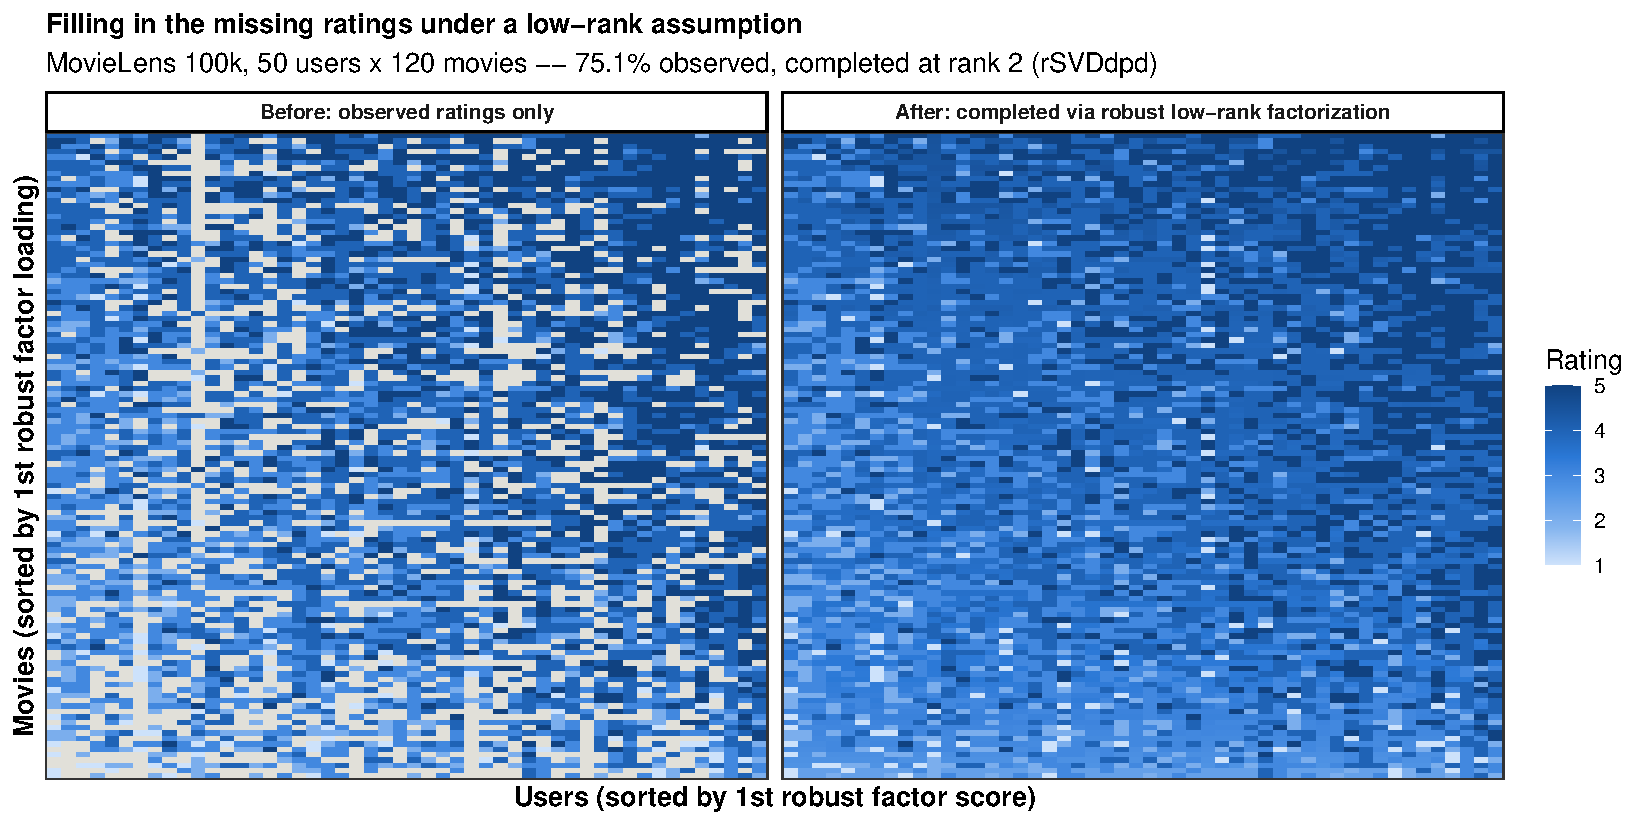
\includegraphics[width = \textwidth]{../../figures/rank_rsvddpd/results_reco_completion.pdf}
    \end{center}
\end{frame}

\begin{frame}{Recommender Systems: Are the Factors Meaningful?}
    \begin{itemize}
        \item A numerically low rank is only useful if the recovered factors correspond to something real -- so look at which movies load most heavily on each robust singular vector.
    \end{itemize}

    \begin{center}
        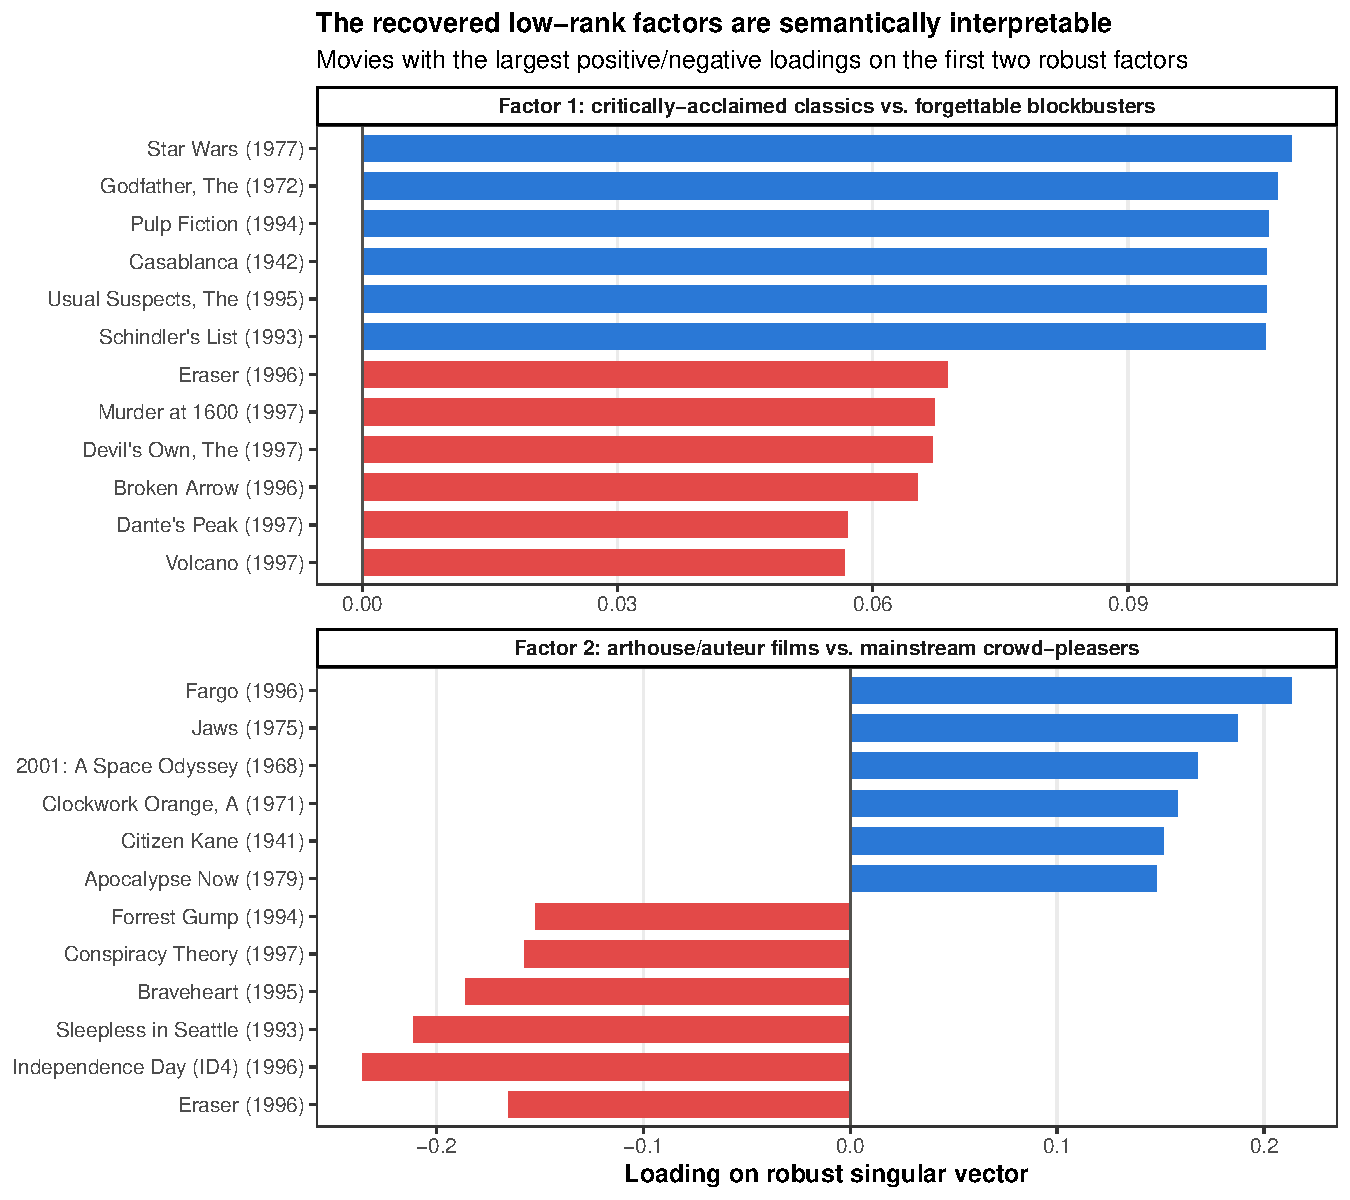
\includegraphics[width = 0.62\textwidth]{../../figures/rank_rsvddpd/results_reco_loadings.pdf}        
    \end{center}
\end{frame}

\begin{frame}{Recommender Systems: Interpreting the Factors}
    \begin{itemize}
        \item Factor 1 separates critically-acclaimed classics (\emph{Godfather}, \emph{Pulp Fiction}, \emph{Casablanca}) from forgettable mid-90s blockbusters (\emph{Volcano}, \emph{Dante's Peak}).
        \pause
        \item Factor 2 separates arthouse/auteur films (\emph{Fargo}, \emph{2001: A Space Odyssey}, \emph{Citizen Kane}) from mainstream crowd-pleasers (\emph{Independence Day}, \emph{Forrest Gump}).
        \pause
        \item[\alert{$\checkmark$}] The robust low-rank structure recovers the ``taste dimensions'' typically found in the recommender-systems literature.
    \end{itemize}
\end{frame}

\begin{frame}{Summary}
    \small
    \begin{itemize}
        \item Rank estimation for noisy matrices has two standard tools -- information criteria and cross-validation -- and \alert{neither is a good fit under contamination}: classical criteria break even with a robust SVD plugged in, and robustified cross-validation is computationally prohibitive.
        \pause
        \item \textbf{DICMR}: a closed-form penalized criterion built on the density power divergence, inheriting robustness directly from the \texttt{rSVDdpd} estimator.
        \pause
        \item Non-asymptotic bounds pin down exactly when DICMR avoids both over- and underestimation, and it is first-order B-robust by construction.
        \pause
        \item Across three very different real datasets -- cross-country bond yields, TCGA gene expression, and MovieLens ratings -- DICMR recovers compact, interpretable, and more accurate low-rank structure than classical or resampling alternatives, at a fraction of the computational cost.
    \end{itemize}
\end{frame}


\begin{frame}[allowframebreaks]{References}
    \tiny
    \begin{thebibliography}{99}
    \bibitem[Hallin and Liška, 2007]{hallin2007determining} Hallin, Marc, and Roman Liška. "Determining the number of factors in the general dynamic factor model." Journal of the American Statistical Association 102, no. 478 (2007): 603-617.
    \bibitem[Basu et al., 1998]{basu1998dpd} Basu, Ayanendranath, Ian R. Harris, Nils L. Hjort, and Michael C. Jones. "Robust and efficient estimation by minimising a density power divergence." Biometrika 85, no. 3 (1998): 549-559.
    \bibitem[Linderman et al., 2022]{linderman2022ALRA} Linderman, George C., Jun Zhao, Manolis Roulis, Piotr Bielecki, Richard A. Flavell, Boaz Nadler, and Yuval Kluger. "Zero-preserving imputation of single-cell RNA-seq data." Nature communications 13, no. 1 (2022): 192.
    \bibitem[Fiorini, 2016]{gene_expression_data} \href{https://doi.org/10.24432/C5R88H}{Fiorini, Samuele. "Gene Expression Cancer RNA-Seq." UCI Machine Learning Repository (2016).}
    \bibitem[Kim et al., 2005]{llsImpute_method} \href{https://doi.org/10.1093/bioinformatics/bth499}{Kim, Hyunsoo, Gene H. Golub, and Haesun Park. "Missing value estimation for DNA microarray gene expression data: local least squares imputation." Bioinformatics 21.2 (2005): 187-198.}
    \bibitem[Li and Li, 2018]{scImpute_method} \href{https://doi.org/10.1038/s41467-018-03405-7}{Li, Wei Vivian, and Jingyi Jessica Li. "An accurate and robust imputation method scImpute for single-cell RNA-seq data." Nature communications 9.1 (2018): 997.}
    \bibitem[van Dijk et al., 2018]{MAGIC_method} \href{https://doi.org/10.1016/j.cell.2018.05.061}{van Dijk, David, et al. "Recovering gene interactions from single-cell data using data diffusion." Cell 174.3 (2018): 716-729.}
    \bibitem[Huang et al., 2018]{SAVER_method} \href{https://doi.org/10.1038/s41592-018-0033-z}{Huang, Mo, et al. "SAVER: gene expression recovery for single-cell RNA sequencing." Nature methods 15.7 (2018): 539-542.}
    \bibitem[Troyanskaya et al., 2001]{knnImpute_method} \href{https://doi.org/10.1093/bioinformatics/17.6.520}{Troyanskaya, Olga, et al. "Missing value estimation methods for DNA microarrays." Bioinformatics 17.6 (2001): 520-525.}
    \bibitem[Roy et al., 2024]{roy2024rsvddpd} Roy, Subhrajyoty, Abhik Ghosh, and Ayanendranath Basu. "Robust singular value decomposition with application to video surveillance background modelling." Statistics and Computing 34.5 (2024): 178.
    \bibitem[Akaike, 1973]{akaike1973information} Akaike, Hirotogu. "Information theory and an extension of the maximum likelihood principle." Selected Papers of Hirotugu Akaike. Springer, New York, NY, 1973. 199-213.
    \bibitem[Schwarz, 1978]{schwarz1978estimating} \href{https://doi.org/10.1214/aos/1176344136}{Schwarz, Gideon. "Estimating the dimension of a model." The Annals of Statistics 6.2 (1978): 461-464.}
    \bibitem[Bai and Ng, 2002]{bai2002determining} \href{https://doi.org/10.1111/1468-0262.00273}{Bai, Jushan, and Serena Ng. "Determining the number of factors in approximate factor models." Econometrica 70.1 (2002): 191-221.}
    \bibitem[Shabalin and Nobel, 2013]{shabalin2013reconstruction} \href{https://doi.org/10.1016/j.jmva.2013.03.005}{Shabalin, Andrey A., and Andrew B. Nobel. "Reconstruction of a low-rank matrix in the presence of Gaussian noise." Journal of Multivariate Analysis 118 (2013): 67-76.}
    \bibitem[Gavish and Donoho, 2014]{gavish2014optimal} Gavish, Matan, and David L. Donoho. "The optimal hard threshold for singular values is $4/\sqrt{3}$." IEEE Transactions on Information Theory 60.8 (2014): 5040-5053.
    \bibitem[Choi et al., 2017]{choi2017selecting} Choi, Yunjin, Jonathan Taylor, and Robert Tibshirani. "Selecting the number of principal components: Estimation of the true rank of a noisy matrix." The Annals of Statistics 45.6 (2017): 2590-2617.
    \bibitem[Xu et al., 2021]{xu2021adaptive} Xu, Zhengqin, Rui He, Shoulie Xie, and Shiqian Wu. "Adaptive rank estimate in robust principal component analysis." Proceedings of the IEEE/CVF Conference on Computer Vision and Pattern Recognition. 2021. 6577-6586.
    \bibitem[Wold, 1978]{wold1978crossvalidation} \href{https://doi.org/10.1080/00401706.1978.10489693}{Wold, Svante. "Cross-validatory estimation of the number of components in factor and principal components models." Technometrics 20.4 (1978): 397-405.}
    \bibitem[Eastment and Krzanowski, 1982]{eastment1982crossvalidation} \href{https://doi.org/10.2307/1267581}{Eastment, H. T., and W. J. Krzanowski. "Cross-validatory choice of the number of components from a principal component analysis." Technometrics 24.1 (1982): 73-77.}
    \bibitem[Gabriel, 2002]{gabriel2002lebiplot} Gabriel, K. Ruben. "Le biplot -- outil d'exploration de données multidimensionnelles." Journal de la Société française de statistique 143.3-4 (2002): 5-55.
    \bibitem[Owen and Perry, 2009]{owen2009bi} \href{https://doi.org/10.1214/08-AOAS227}{Owen, Art B., and Patrick O. Perry. "Bi-cross-validation of the SVD and the nonnegative matrix factorization." The Annals of Applied Statistics 3.2 (2009): 564-594.}
    \bibitem[Arciniegas-Alarcón et al., 2022]{alarcon2022cv} \href{https://doi.org/10.3390/asi5040069}{Arciniegas-Alarcón, Sergio, Marisol García-Peña, and Wojtek J. Krzanowski. "Cross-validation for lower rank matrices containing outliers." Applied System Innovation 5.4 (2022): 69.}
    \bibitem[Thorndike, 1953]{thorndike1953elbow} \href{https://doi.org/10.1007/BF02289263}{Thorndike, Robert L. "Who belongs in the family?" Psychometrika 18.4 (1953): 267-276.}
    \bibitem[Hoff, 2007]{hoff2007model} Hoff, Peter D. "Model averaging and dimension selection for the singular value decomposition." Journal of the American Statistical Association 102.478 (2007): 674-685.
    \bibitem[Mazumder et al., 2010]{mazumder2010spectral} Mazumder, Rahul, Trevor Hastie, and Robert Tibshirani. "Spectral regularization algorithms for learning large incomplete matrices." The Journal of Machine Learning Research 11 (2010): 2287-2322.
    \end{thebibliography}
\end{frame}


% =======
% Thanks

% \thanksframe{Thank You!}

\begin{frame}{Thank You / Questions?}
    \begin{center}
        \textbf{Subhrajyoty Roy} \\ 
        \texttt{roy.s@wustl.edu} \\
        \vspace{0.3em}
        % \small in collaboration with Abhik Ghosh and Ayanendranath Basu
    \end{center}

    \vspace{1em}
    \begin{center}
        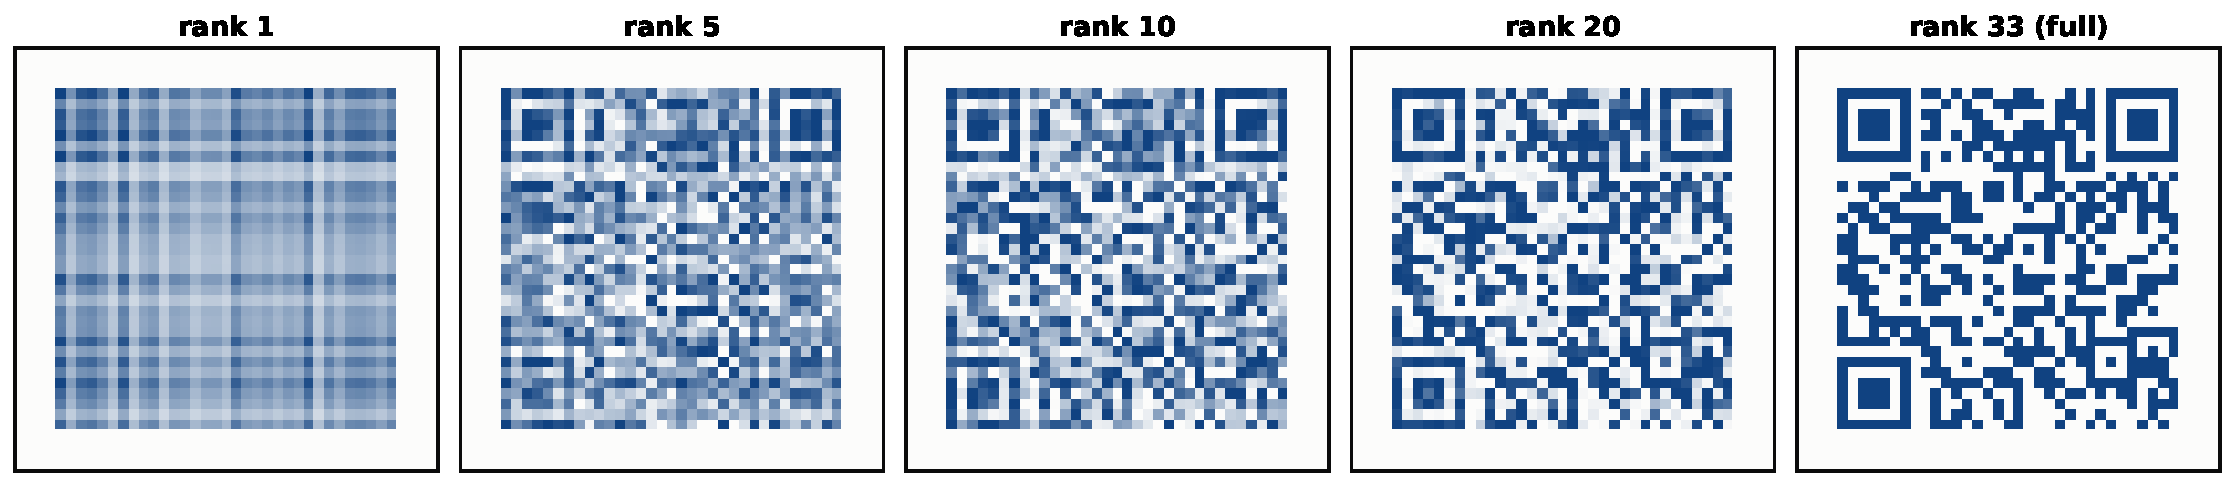
\includegraphics[width = \textwidth]{../../figures/rank_rsvddpd/qr_lowrank_reveal.pdf}

        \vspace{0.3em}
        \small Paper: \url{https://arxiv.org/abs/2510.19583}
    \end{center}
\end{frame}


\end{document}
